\documentclass[tikz,border=1mm]{standalone}
\usepackage{xcolor}

\begin{document}
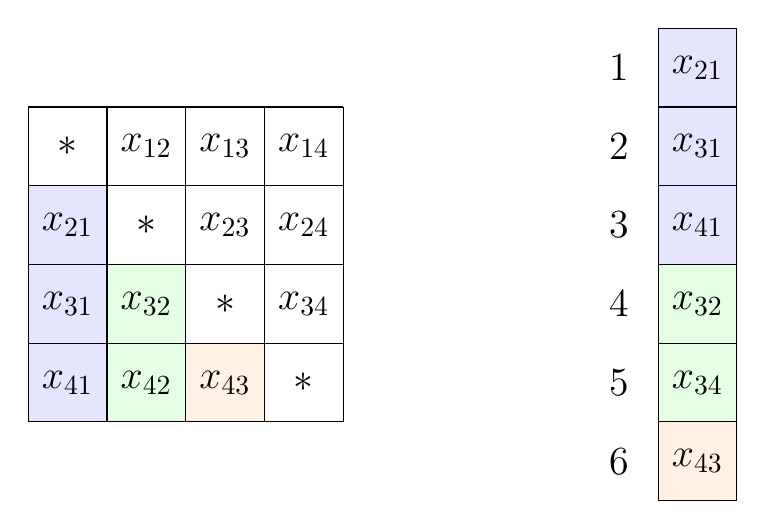
\begin{tikzpicture}[minimum width = 1cm, minimum height = 1cm, font = \Large]
  %%% matrix representation %%%
  % row 1
  \node at (0.5,3.5) {$\ast$};
  \node at (1.5,3.5) {$x_{12}$};
  \node at (2.5,3.5) {$x_{13}$};
  \node at (3.5,3.5) {$x_{14}$};
  % row 2
  \node[fill=blue!10] at (0.5,2.5) {$x_{21}$};
  \node at (1.5,2.5) {$\ast$};
  \node at (2.5,2.5) {$x_{23}$};
  \node at (3.5,2.5) {$x_{24}$};
  % row 3
  \node[fill=blue!10] at (0.5,1.5) {$x_{31}$};
  \node[fill=green!10] at (1.5,1.5) {$x_{32}$};
  \node at (2.5,1.5) {$\ast$};
  \node at (3.5,1.5) {$x_{34}$};
  % row 4
  \node[fill=blue!10] at (0.5,0.5) {$x_{41}$};
  \node[fill=green!10] at (1.5,0.5) {$x_{42}$};
  \node[fill=orange!10] at (2.5,0.5) {$x_{43}$};
  \node at (3.5,0.5) {$\ast$};
  % add a grid
  \draw[step=1cm] (0,0) grid (4,4);

  %%% trivec representation %%%
  % from column 1
  \node[fill=blue!10] at (8.5,4.5) {$x_{21}$};
  \node[fill=blue!10] at (8.5,3.5) {$x_{31}$};
  \node[fill=blue!10] at (8.5,2.5) {$x_{41}$};
  % from column 2
  \node[fill=green!10] at (8.5,1.5) {$x_{32}$};
  \node[fill=green!10] at (8.5,0.5) {$x_{34}$};
  % from column 3
  \node[fill=orange!10] at (8.5,-0.5) {$x_{43}$};
  % add a grid
  \draw[step=1cm] (8,-1) grid (9,5);
  % add indices
  \node at (7.5,+4.5) {1};
  \node at (7.5,+3.5) {2};
  \node at (7.5,+2.5) {3};
  \node at (7.5,+1.5) {4};
  \node at (7.5,+0.5) {5};
  \node at (7.5,-0.5) {6};
\end{tikzpicture}
\end{document}